\subsection{Kinematics}
\label{kinematics}

\label{EXP}
We propose to measure the tensor asymmetry $A_{zz}$ for $\XMIN<x<\XMAX$, $\QMIN$~(GeV/$c)^2 < Q^2 <\QMAX$~(GeV/$c)^2$, and $\WMIN < W_{NN} < \WMAX$~GeV and extract the tensor analyzing power $T_{20}$ for $\QMINT20$~(GeV/$c)^2 < Q^2 <\QMAXT20$~(GeV/$c)^2$. Central kinematics of the spectrometers are given in Table~\ref{RATES1}
%, estimates for the uncertainties of $A_{zz}$ are given in Tables~\ref{RATES2}-\ref{RATES3}, and estimates for the uncertainties of $T_{20}$ are given in Table\need
. Fig.~\ref{kincov} shows the planned kinematic coverage utilizing the Hall C HMS and SHMS spectrometers at forward angles. 

\begin{table}
\begin{center}
\begin{tabular}{cc|c|c|c|c|c|c}
 & & $E_0$ & $Q^2$    	& $E'$  &    $\theta_{e'}$  &  Rates   & PAC Time   \\
%& (GeV) & (GeV$^2$)  & (GeV)  &     (deg.)   &   (kHz)  & (hours) \\
& & (GeV) & (GeV$^2$)  & (GeV)  &     ($^{\circ}$)   &   (kHz)  & (Days) \\
%\multicolumn{2}{|c|}{$\times 10^{-2}$}
\hline\hline
SHMS & (S1) & 8.8	&  1.5	&  8.36	&    8.2  	&    0.38	&   25 \\
HMS  & (H1) & 8.8	&  2.9	&  7.26	&    12.2	&    0.04	&   25 \\  
SHMS & (S2) & 6.6	&  0.7	&  6.35	&    7.5 	&    3.57	&   8 \\
HMS  & (H2) & 6.6	&  1.8	&  5.96	&    12.3	&    0.09	&   8 \\  
SHMS & (S3) & 2.2	&  0.2	&  2.15	&    10.9 	&    10.5	&   1 \\
HMS  & (H3) & 2.2	&  0.3	&  2.11	&    14.9	&    3.23	&   1 \\  
\hline\hline
\end{tabular}
\caption{\label{RATES1}Summary of the central kinematics and physics rates using the Hall C  spectrometers.}
\end{center}
\end{table}









\begin{figure}
\begin{center}
%\includegraphics[width=\textwidth]{figs/Pzz_30_all_q2_w.eps}
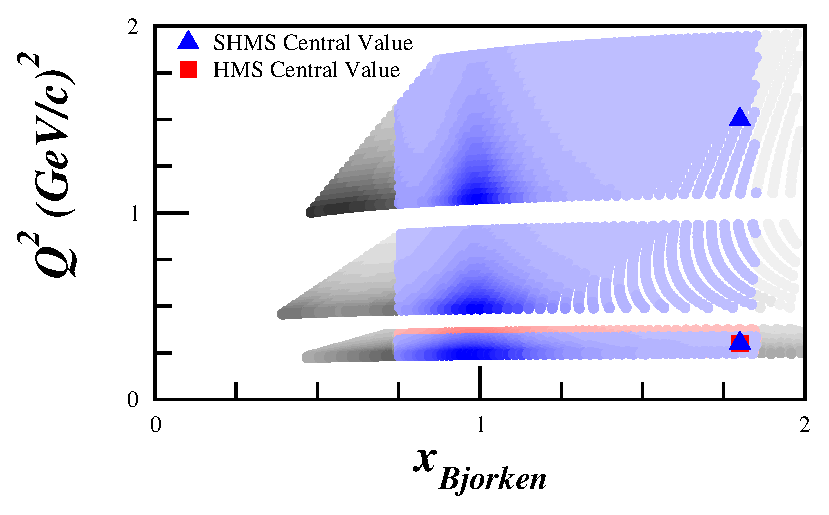
\includegraphics[width=0.49\textwidth]{figs/Pzz_30_all_q2.eps}

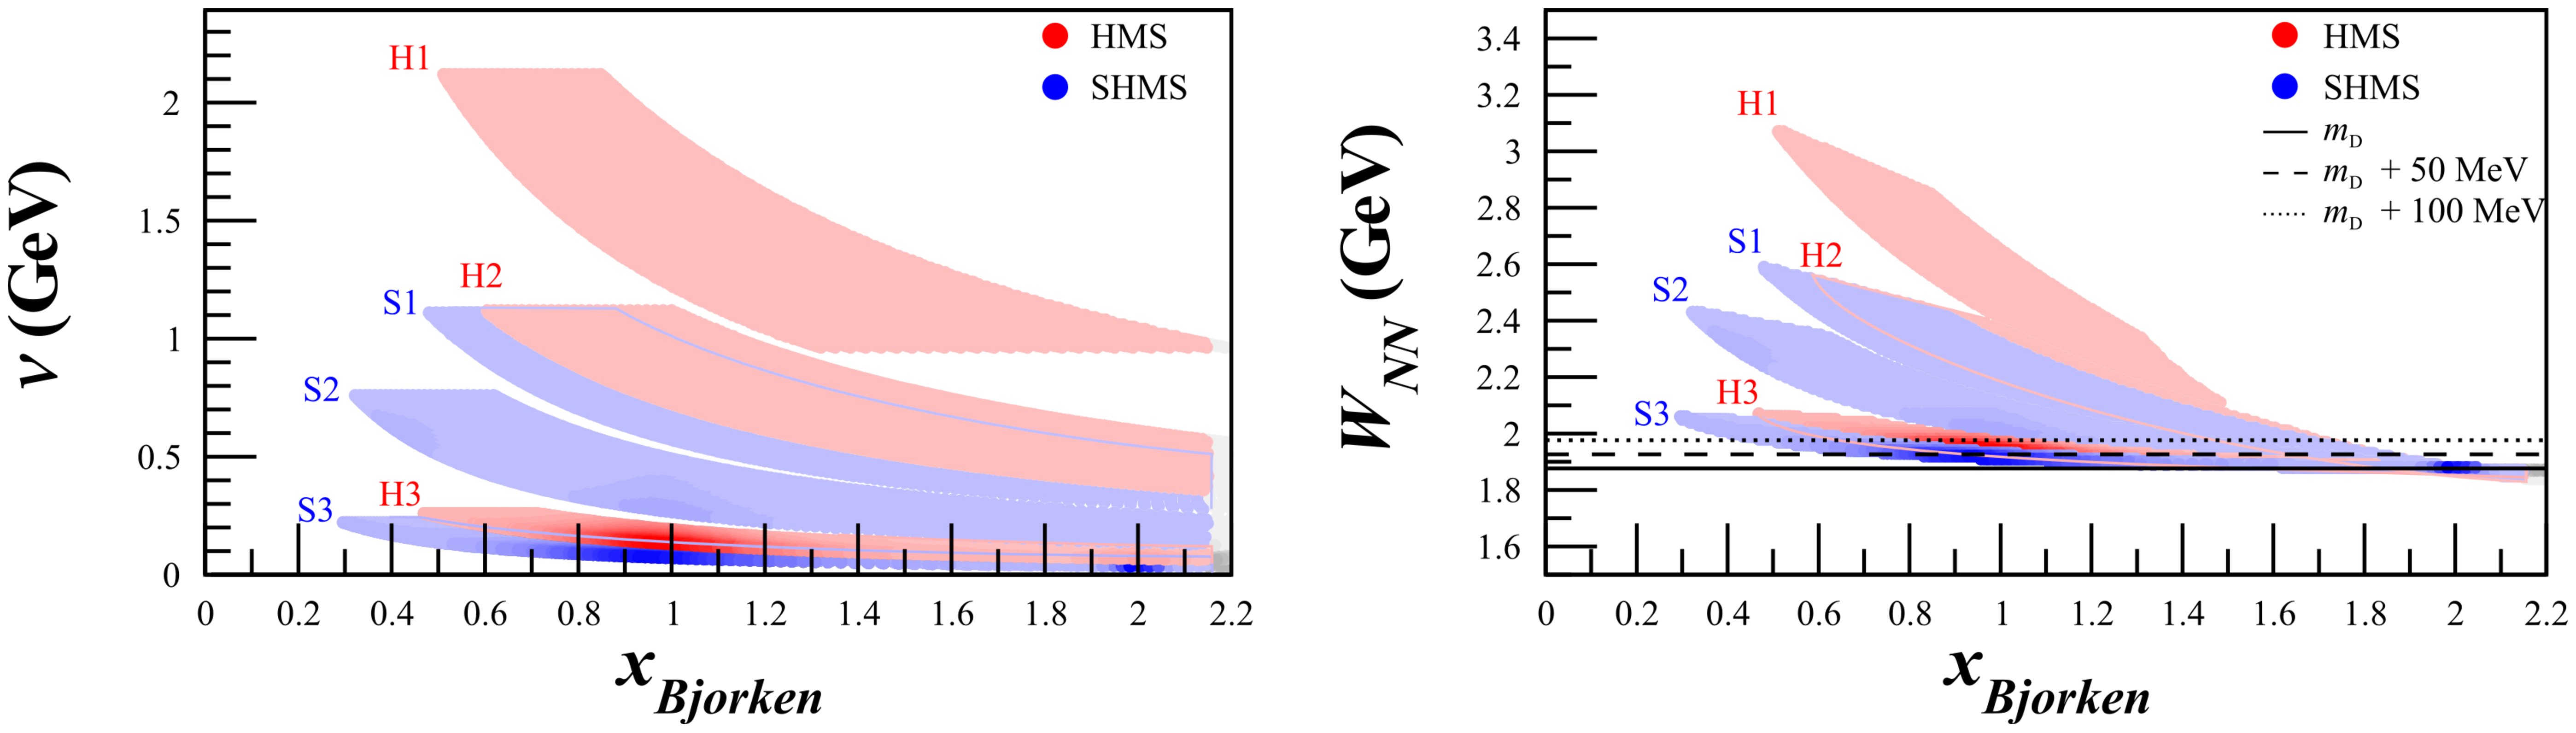
\includegraphics[width=\textwidth]{figs/Pzz_30_all_nu_wnn.eps}
%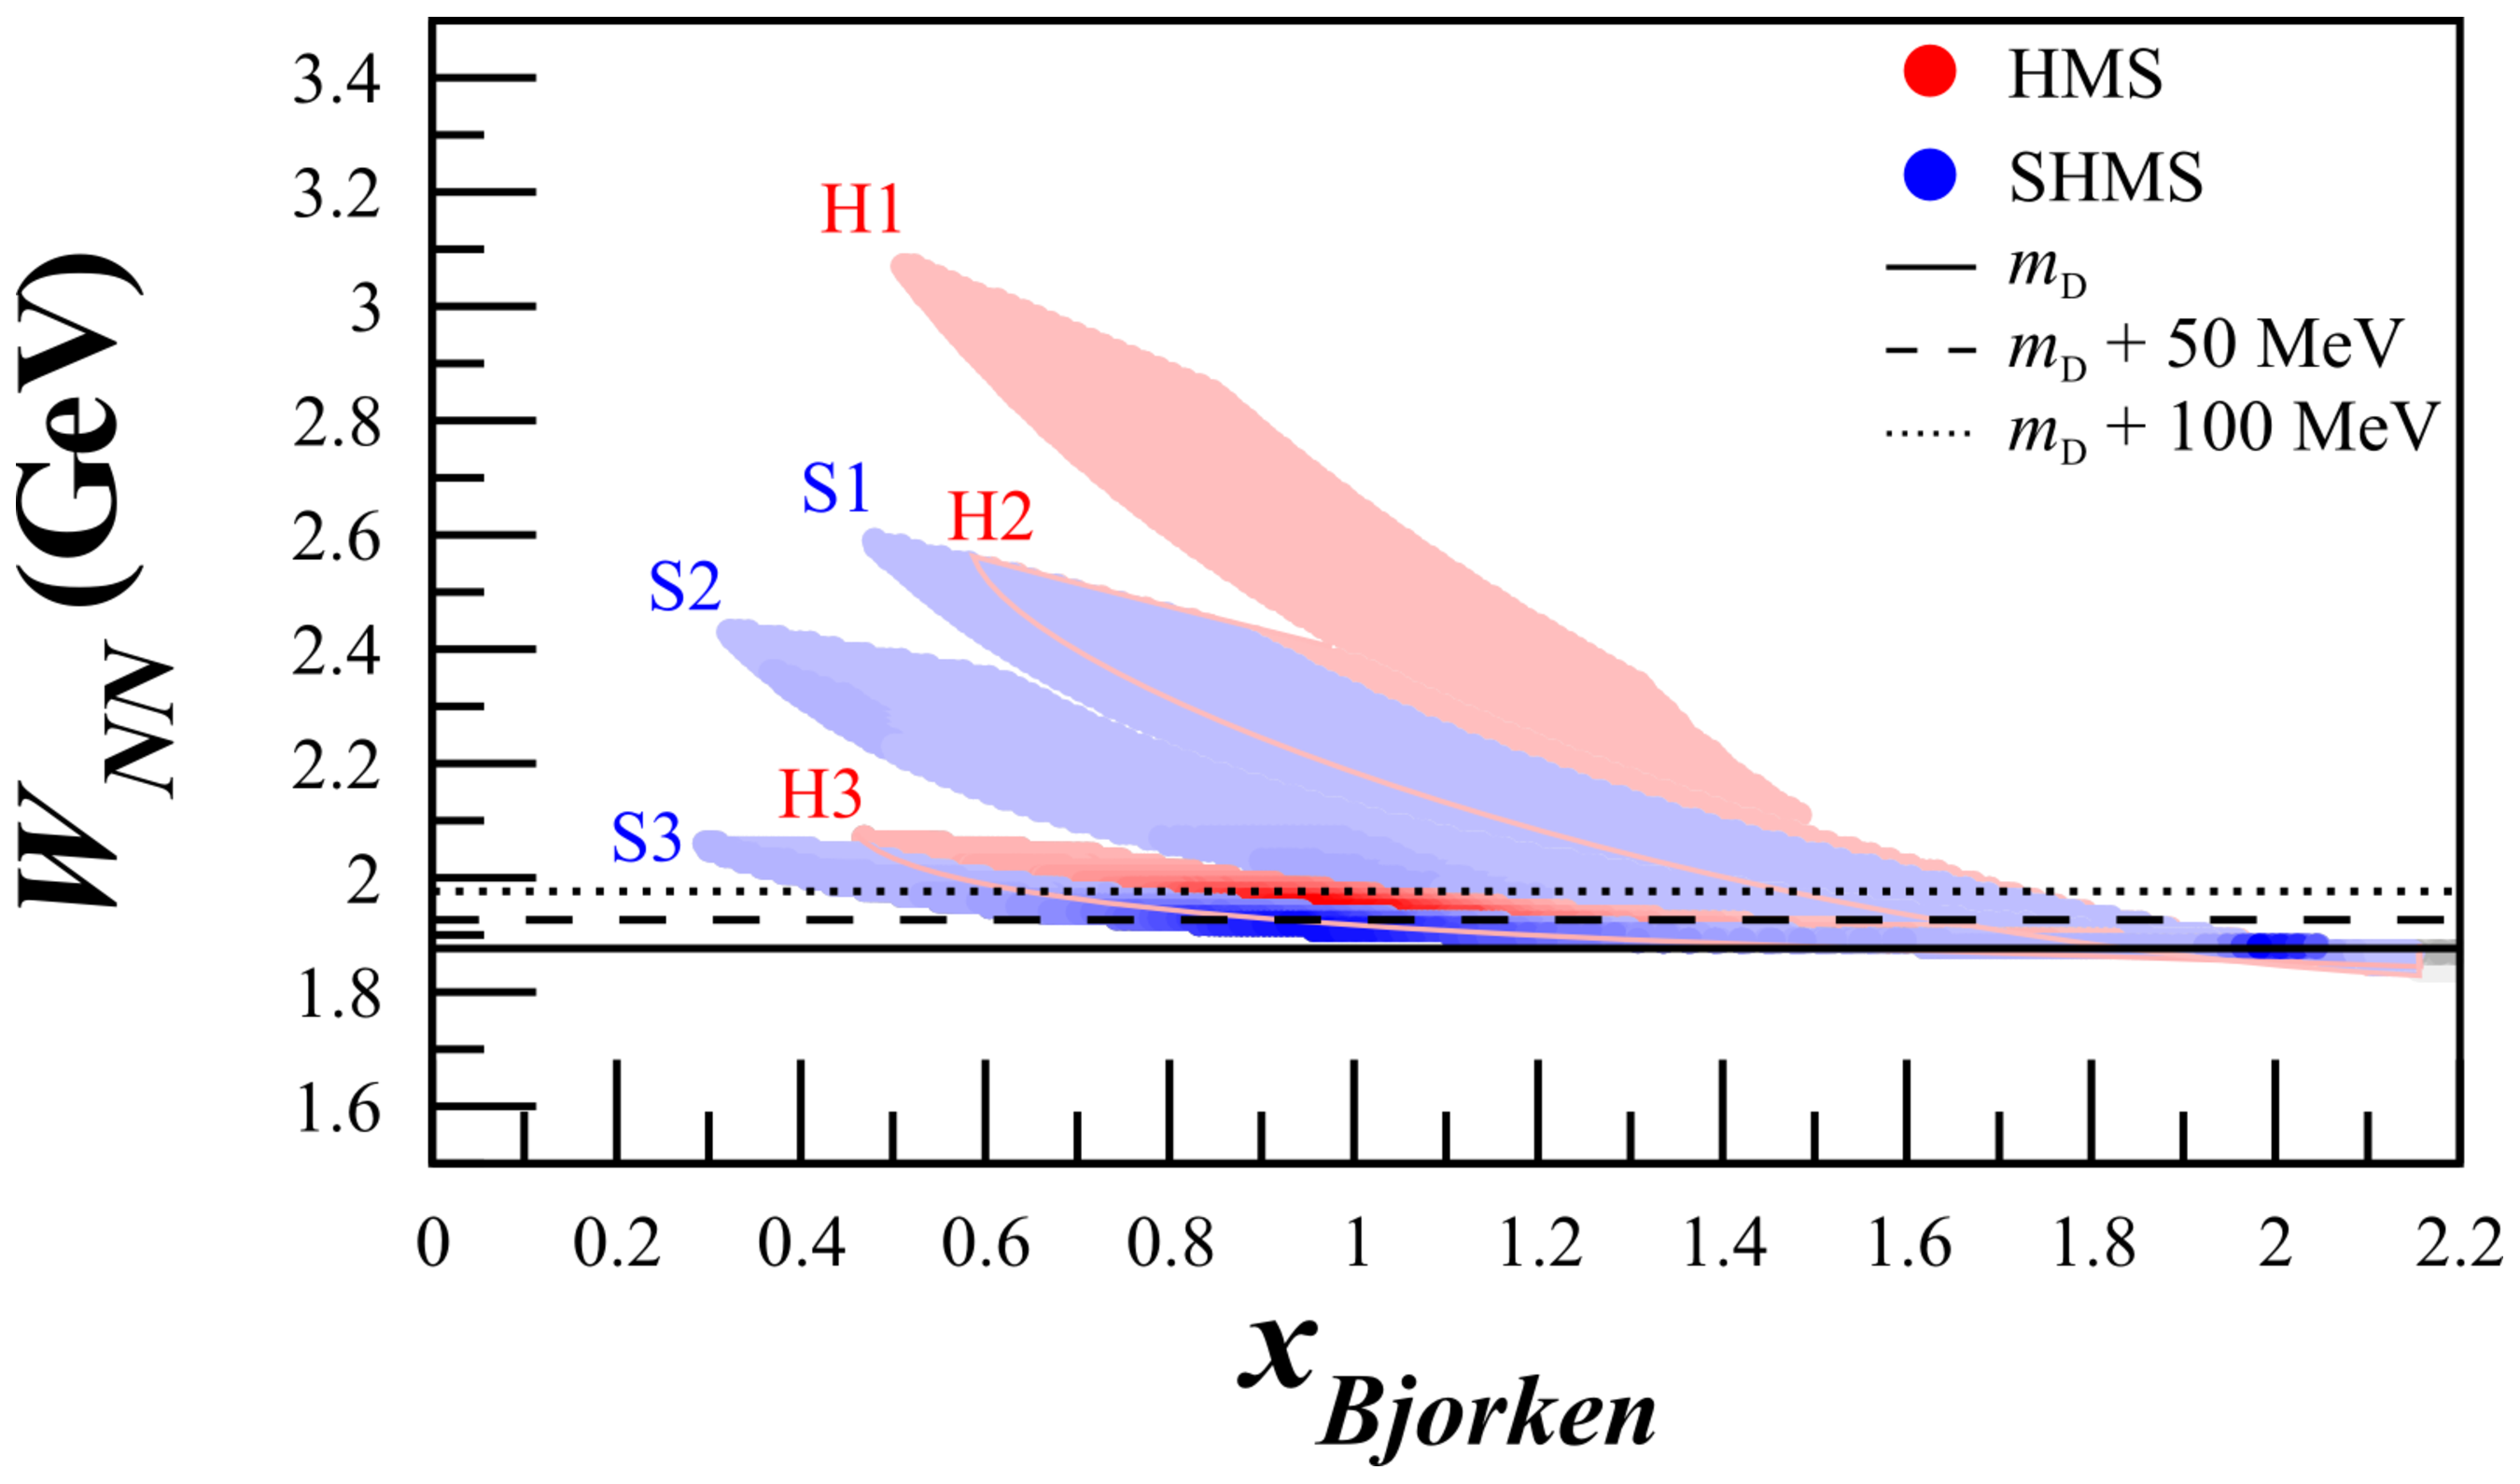
\includegraphics[width=0.49\textwidth]{figs/Pzz_30_all_wnn.eps} %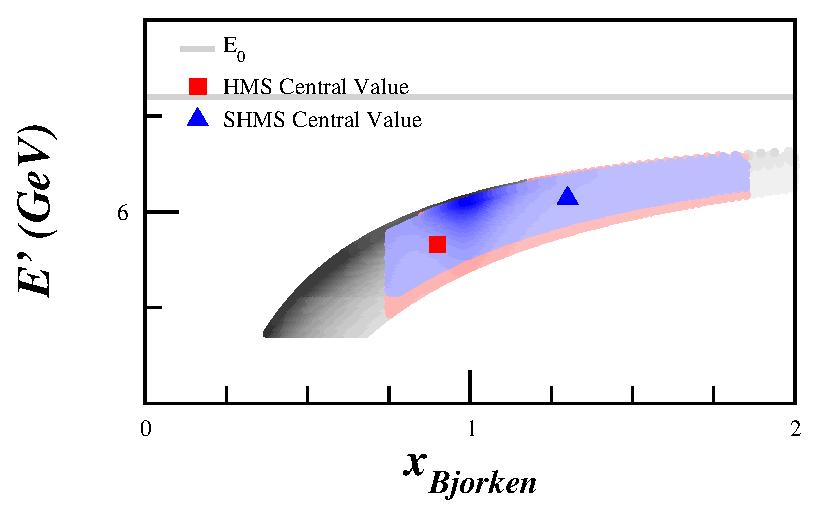
\includegraphics[width=0.49\textwidth]{figs/kine/Pzz_30_eprime.eps}
%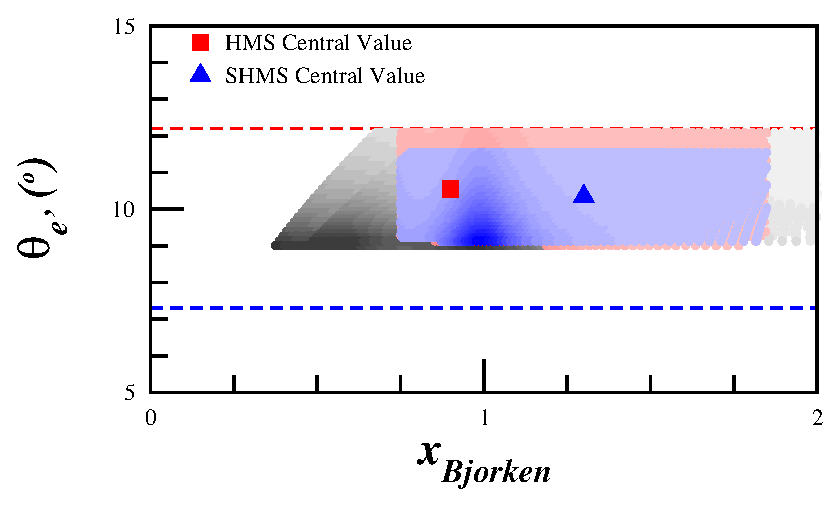
\includegraphics[width=0.49\textwidth]{figs/kine/Pzz_30_theta_eprime.eps}~~ 

\caption{\label{kincov} Kinematic coverage for central spectrometer settings at $Q^2=2.9~(\mathrm{GeV}/c)^2$ (H1), $1.8~(\mathrm{GeV}/c)^2$ (H2), $1.5~(\mathrm{GeV}/c)^2$ (S1), $0.7~(\mathrm{GeV}/c)^2$ (S2), $0.3~(\mathrm{GeV}/c)^2$ (H3), and $0.2~(\mathrm{GeV}/c)^2$ (S3). The grey regions are not included in our statistics estimates since they fall outside the range of electron-deuteron scattering. Darker shading represents areas with higher statistics. The solid, dashed, and dotted lines in the $W_{NN}$ plot indicate deuteron mass, deuteron mass + 50 MeV, and deuteron mass + 100 MeV, respectively. Virtual-nucleon and light cone calculations are only valid for $W_{NN}>m_D+50$~MeV.}
\end{center}
\end{figure}

Although it has been pointed out that the current construction of the SHMS constrains it to angles $>10\%$ due to fringe fields affecting the beam entering the dump~\cite{Moore:2014sxa}, this can be resolved in a number of ways. As discussed in \cite{Moore:2014sxa}, passive iron shielding can be installed within the SHMS that would not affect the target field. Additionally, given the low beam current proposed, a local beam dump could be installed immediately following the target. In the worst case, we could meet the physics motivation by keeping the same $Q^2$ ranges as S1, S2, and S3 but lowering the highest beam energies while putting the SHMS at larger angles. In this case, the HMS would be used at very similar angles to combine statistics between the spectrometers to make up for the loss in statistics from the SHMS. 


The polarized \TARGET target is discussed in Section~\ref{POLTARGSEC}.  The magnetic field of the target will be held constant along the beamline at all times, while the target state is alternated between a polarized and unpolarized state.
The tensor polarization and packing fraction used in the rates estimate are \PZZ\% and \PF, respectively. 
The dilution factor in the range of this measurement is shown in Fig.~\ref{fdil_plot}. The spread of the elastic peak for the dilution factor was calculated assuming a momentum resolution of $0.1\%$ for the HMS and $0.08\%$ for the SHMS.
With an incident electron beam current of \CURRENT nA, the expected deuteron luminosity is \LUMI.


%$1.57\times 10^{35}$~cm$^{-2}}$s$^{-1}$.
%$?.??\times 10^{35}$~cm$^{-2}$s$^{-1}$.

\begin{figure}
\begin{center}
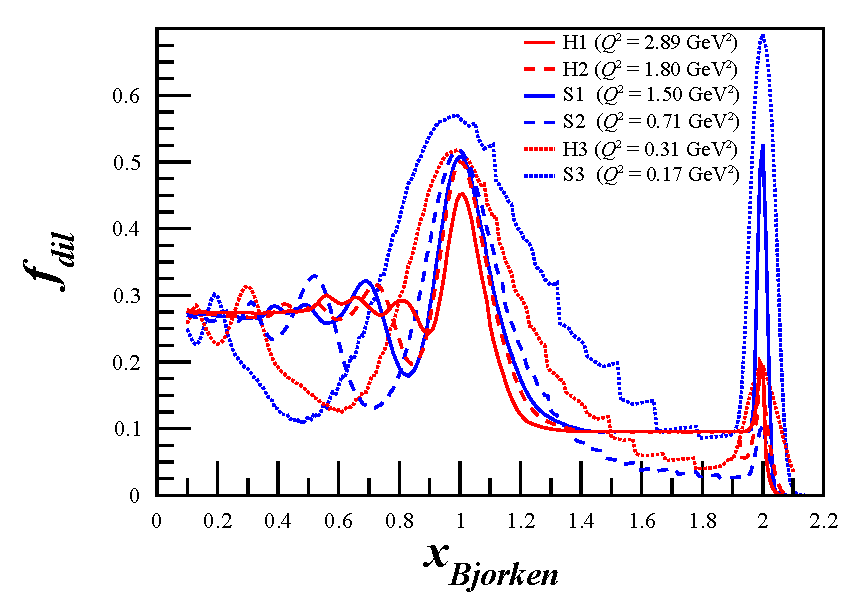
\includegraphics[width=0.65\textwidth]{figs/Pzz_30_fdil_all.eps} 
\caption{\label{fdil_plot}Projected dilution factor covering the entire $x$ range to be measured using a combination of P. Bosted's~\cite{Bosted:2012qc} and M. Sargsian's~\cite{misak-convo} code, along with a calculation of the elastic peak using a parametrization of the deuteron form factors, for the SHMS and HMS.}
\end{center}
\end{figure}


The momentum bite and the acceptance were assumed to be $\Delta P = \pm 8\%$ and $\Delta\Omega = 5.6$~msr for the HMS, and $\Delta P= ^{+20\%}_{-8\%}$ 
%$-8<\Delta P <+20\%$
and $\Delta\Omega =4.4$~msr for the SHMS. 
%
For the choice of the kinematics,
special attention was taken onto the angular and momentum limits of the spectrometers with a longitudinal polarized target: for the
HMS, $12.2^{\circ} \le \theta \le 85^{\circ}$ and $1 \le P_0 \le 7.3$ GeV/c, and for the SHMS,
$5.5^{\circ} \le \theta \le 40^{\circ}$ and $2 \le P_0 \le 11$ GeV/c. In addition, the
opening angle between the spectrometers is physically constrained to be larger than 17.5$^{\circ}$.

A total of \productiondays days of beam time is requested for production data, with an additional \overheaddays days of expected overhead. The expected uncertainties, described in detail in Section~\ref{uncertainties}, are given in Tables~\ref{RATES2}-\ref{RATES-T20} and Figs.~\ref{PROJ}-\ref{PROJ-T20}.

\begin{table}
\begin{center}
\begin{tabular}{c|ccc|ccc|ccc}
 ~ & \multicolumn{3}{|c}{H1: $Q^2=2.9\mathrm{~(GeV/}c)^2$} & \multicolumn{3}{|c}{H2: $Q^2=1.8\mathrm{~(GeV/}c)^2$} & \multicolumn{3}{|c}{S1: $Q^2=1.5\mathrm{~(GeV/}c)^2$} \\
 \hline
  $x$  & $f_{dil}$ & $\delta A_{zz}^{stat}$ & $\delta A_{zz}^{sys}$ & $f_{dil}$ & $\delta A_{zz}^{stat}$ & $\delta A_{zz}^{sys}$ & $f_{dil}$ & $\delta A_{zz}^{stat}$ & $\delta A_{zz}^{sys}$ \\
  &     & $\times 10^{-2}$  & $\times 10^{-2}$  &    & $\times 10^{-2}$  & $\times 10^{-2}$ &    & $\times 10^{-2}$  & $\times 10^{-2}$ \\
\hline\hline
%       |         Q2=2.9         |      Q2=1.8           |      Q2=1.5
%  x  	   fdil 	   dAzz	 dAzzSys  fdil 	  dAzz   dAzzSys  fdil   dAzz	 dAzzSys
 0.50   &  0.29	 & 2.02	& 1.84	& ---	& ---	& ---	& 0.25	& 0.72	& 1.84 \\
 0.60   &  0.29	 & 0.91	& 0.10	& 0.27	& 3.15	& 0.10	& 0.30	& 0.36	& 0.10 \\ 
 0.70   &  0.27	 & 1.01	& 0.10	& 0.32	& 1.26	& 0.10	& 0.29	& 0.38	& 0.10 \\
 0.80	&  0.30	 & 1.11	& 1.34	& 0.20	& 2.00	& 0.48	& 0.17	& 0.74	& 1.34 \\
 0.90	&  0.24	 & 1.73 	& 0.38 	& 0.27	& 1.45	& 1.10	& 0.29	& 0.44	& 0.38 \\
 1.00	&  0.46	 & 1.03	& 0.10 	& 0.50	& 0.74	& 0.10	& 0.51	& 0.24	& 0.10 \\
 1.10	&  0.28	 & 2.48	& 0.14 	& 0.33	& 1.58	& 1.65	& 0.34	& 0.49	& 0.14 \\
 1.20	&  0.09	 & 11.7	& 1.55 	& 0.10	& 7.18	& 3.31	& 0.17	& 1.34	& 1.55 \\
 1.30	&  0.11	 & 16.8	& 4.13 	& 0.11	& 9.76	& 4.96	& 0.12	& 2.79	& 4.13 \\
 1.40	&  ---	 & ---	& --- 	& 0.12	& 15.1	& 6.65	& 0.13	& 4.30	& 6.72 \\
 1.50	&  ---	 & ---	& ---	& 0.11	& 19.8	& 8.29	& 0.10	& 7.01	& 8.34 \\
 1.60	&  ---	 & ---	& --- 	& ---	& ---	& ---	& 0.10	& 9.60	& 8.42 \\
 1.70	&  ---	 & ---	& --- 	& ---	& ---	& ---	& 0.10	& 12.7	& 7.04 \\
 1.80	&  ---	 & ---	& --- 	& ---	& ---	& ---	& 0.10	& 16.6	& 4.72 \\
 2.00   &  ---	 & ---	& ---	& 0.20	& 9.33	& 9.20	& 0.50	& 2.79	& 9.20 \\
\hline\hline
\end{tabular}
\caption{\label{RATES2}Summary of the expected uncertainty for each $x$ bin for settings S1, H1, and H2. }
\end{center}
\end{table}

\begin{table}
\begin{center}
\begin{tabular}{c|ccc|ccc|ccc}
 ~ & \multicolumn{3}{|c}{S2: $Q^2=0.7\mathrm{~(GeV/}c)^2$} & \multicolumn{3}{|c}{H3: $Q^2=0.3\mathrm{~(GeV/}c)^2$} & \multicolumn{3}{|c}{S3: $Q^2=0.2\mathrm{~(GeV/}c)^2$} \\
 \hline
  $x$  & $f_{dil}$ & $\delta A_{zz}^{stat}$ & $\delta A_{zz}^{sys}$ & $f_{dil}$ & $\delta A_{zz}^{stat}$ & $\delta A_{zz}^{sys}$ & $f_{dil}$ & $\delta A_{zz}^{stat}$ & $\delta A_{zz}^{sys}$ \\
  &     & $\times 10^{-2}$  & $\times 10^{-2}$  &    & $\times 10^{-2}$  & $\times 10^{-2}$ &    & $\times 10^{-2}$  & $\times 10^{-2}$ \\
\hline\hline
%       |         Q2=0.7         |      Q2=0.3           |      Q2=0.2
%  x  	   fdil 	   dAzz	 dAzzSys  fdil 	  dAzz   dAzzSys  fdil   dAzz	 dAzzSys
 0.30   &  0.24	 & 0.99	& 1.84	& ---	& ---	& ---	& 0.18	& 2.13	& 1.84 \\
 0.40   &  0.28	 & 0.26	& 1.84	& ---	& ---	& ---	& 0.12	& 1.38	& 1.84 \\
 0.50   &  0.32	 & 0.21	& 1.84	& 0.14	& 3.52	& 1.84	& 0.11	& 1.23	& 1.84 \\
 0.60   &  0.19	 & 0.41	& 0.10	& 0.12	& 2.26	& 0.10	& 0.18	& 0.78	& 0.10 \\ 
 0.70   &  0.13	 & 0.68	& 0.10	& 0.18	& 1.33	& 0.10	& 0.28	& 0.48	& 0.10 \\
 0.80	&  0.19	 & 0.48	& 0.48	& 0.30	& 0.72	& 0.48	& 0.42	& 0.31	& 0.48 \\
 0.90	&  0.39	 & 0.22 	& 1.10 	& 0.46	& 0.45	& 1.10	& 0.54	& 0.24	& 1.10 \\
 1.00	&  0.52	 & 0.16	& 0.10 	& 0.52	& 0.43	& 0.10	& 0.58	& 0.25	& 0.10 \\
 1.10	&  0.39	 & 0.28	& 1.27 	& 0.43	& 0.63	& 1.07	& 0.53	& 0.33	& 0.95 \\
 1.20	&  0.22	 & 0.65	& 2.54 	& 0.30	& 1.15	& 2.14	& 0.40	& 0.55	& 1.91 \\
 1.30	&  0.14	 & 1.34	& 3.81 	& 0.19	& 2.16	& 3.22	& 0.32	& 0.83	& 2.87 \\
 1.40	&  0.09	 & 2.29	& 5.06 	& 0.14	& 3.52	& 4.29	& 0.24	& 1.31	& 3.82 \\
 1.50	&  0.06	 & 4.09	& 6.35	& 0.10	& 5.85	& 5.37	& 0.20	& 1.86	& 4.78 \\
 1.60	&  0.04	 & 7.76	& 7.60 	& 0.06	& 10.4	& 6.45	& 0.14	& 2.87	& 5.74 \\
 1.70	&  0.04	 & 9.23	& 8.88 	& 0.05	& 13.5	& 7.52	& 0.10	& 4.53	& 6.69 \\
 1.80	&  0.03	 & 14.9	& 9.20 	& 0.06	& 13.9	& 8.60	& 0.11	& 4.73	& 7.66 \\
 2.00   &  0.67	 & 3.79	& 9.20	& 0.20	& 3.05	& 9.20	& 0.70	& 0.45	& 9.20 \\
\hline\hline
\end{tabular}
\caption{\label{RATES3}Summary of the expected uncertainty for each $x$ bin for settings S2, S3, and H3. }
\end{center}
\end{table}


\begin{figure}
\begin{center}
%\includegraphics[width=0.45\textwidth]{figs/plots0705/b1_proj_newmiller_lin.eps}
%\hspace{0.5cm}
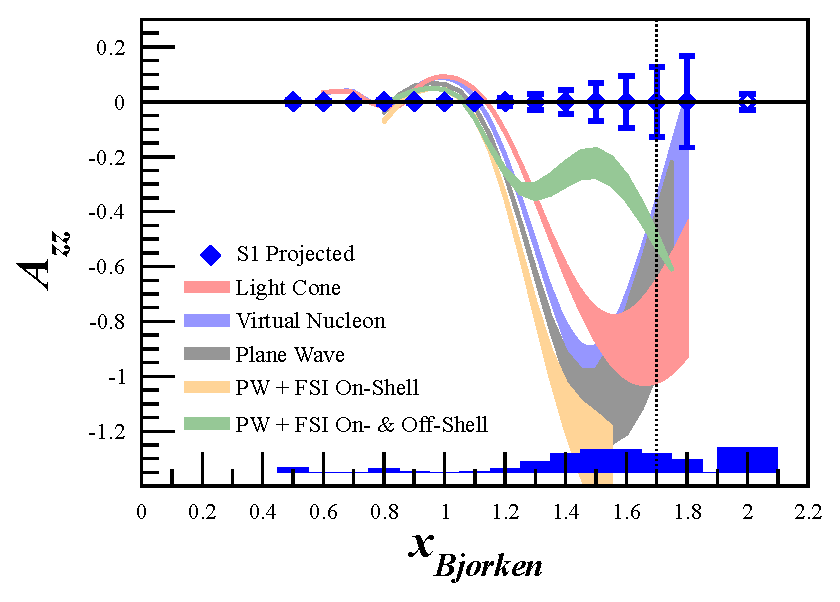
\includegraphics[width=0.49\textwidth]{figs/Azz_S1.eps}
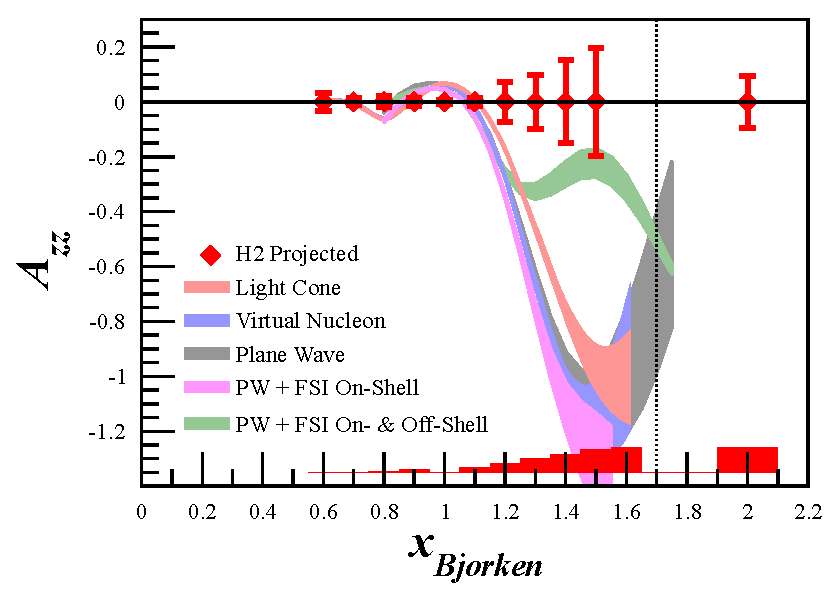
\includegraphics[width=0.49\textwidth]{figs/Azz_H2.eps}
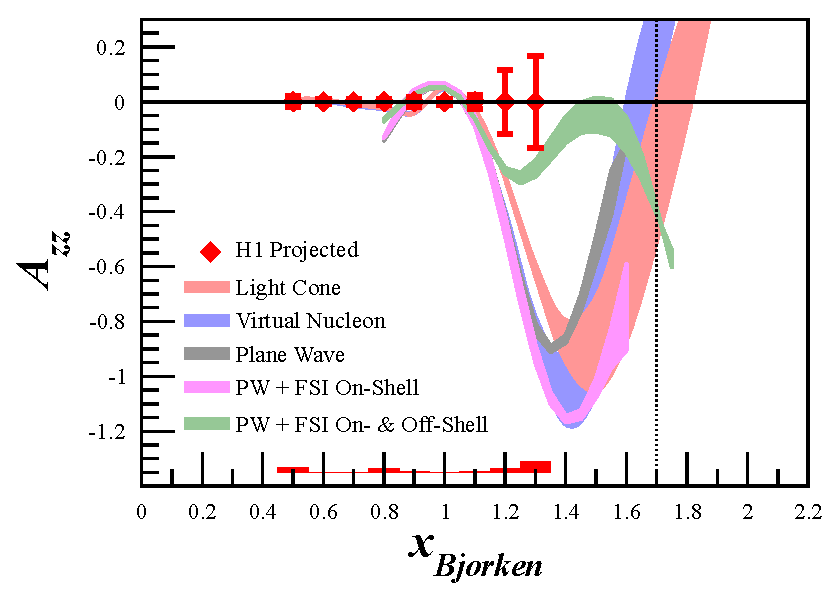
\includegraphics[width=0.49\textwidth]{figs/Azz_H1.eps}
 %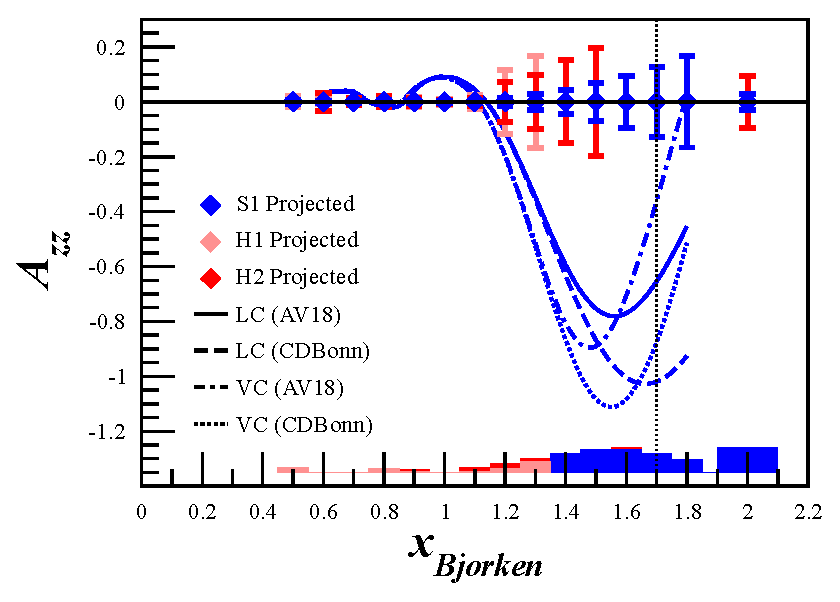
\includegraphics[width=0.49\textwidth]{figs/Azz_S1_H1_H2_vn_lc.eps} 
%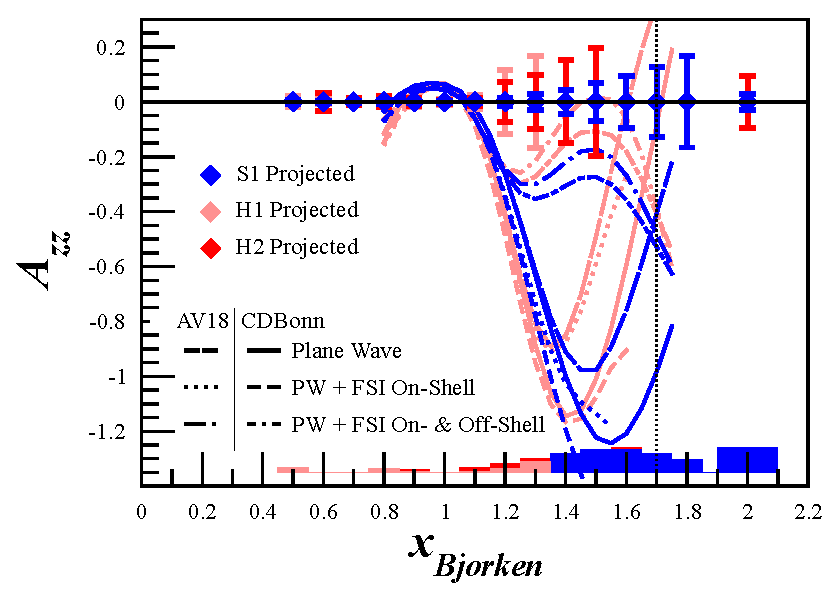
\includegraphics[width=0.49\textwidth]{figs/Azz_S1_H1_H2_fsi.eps} \\
\includegraphics[width=0.49\textwidth]{figs/Azz_S2_H3_S3.eps} 
\caption{\label{PROJ}Projected uncertainties for the tensor asymmetry $A_{zz}$ with \productiondays days of beam time for SHMS settings S1, S2, and S3, and HMS settings H1, H2, and H2 as described in Table~\ref{RATES1}. The bottom band represents the systematic uncertainty. The bands for the theoretical calculations show the spread based on the choice of NN potentials. The upper $x$ limit for H1 (H2) is $x=1.3$ ($x=1.5$). Light-cone (LC) and virtual-nucleon (VN) calculations using the AV18 and CDBonn potentials were provided by M. Sargsian~\cite{Sargsian:2014fla}. The dotted line at $x=1.75$ indicates the threshold of $W_{NN}>m_D+50$~MeV where LC and VN calculations begin to not be valid as $A_{zz}$ approaches the elastic peak~\cite{Frankfurt:1993sp}. Final state interactions on the virtual-nucleon model were provided by W. Cosyn~\cite{cosyn-convo}, indicating the effects from on- and off-shell. The bottom-right plot includes a modified Frankfurt and Strikman model~\cite{Frankfurt:1988nt} that estimates the peak shifts in $x$ expected due to the SRC scaling changing with $Q^2$~\cite{Frankfurt:2008zv}.
}
\end{center}
\end{figure}

\begin{figure}
\begin{center}
%\includegraphics[width=0.45\textwidth]{figs/plots0705/b1_proj_newmiller_lin.eps}
%\hspace{0.5cm}
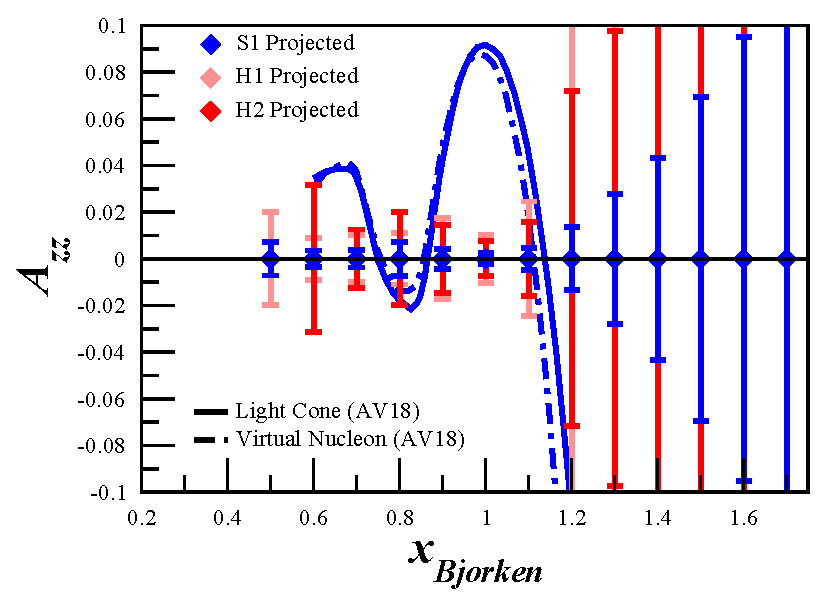
\includegraphics[width=0.49\textwidth]{figs/Azz_S1_H1_H2_zoom.eps} 
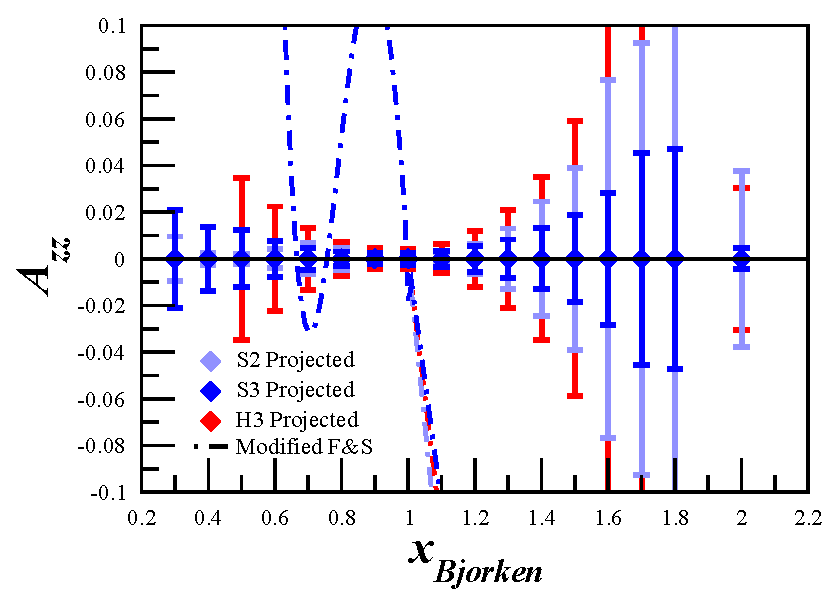
\includegraphics[width=0.49\textwidth]{figs/Azz_S2_H3_S3_zoom.eps} 
\caption{\label{PROJ-zoom}Projected uncertainties for the tensor asymmetry $A_{zz}$ with \productiondays days of beam time, same as in Figure~\ref{PROJ}, but zoomed in to $-0.1<A_{zz}<0.1$ to more clearly show the small uncertainties around the quasi-elastic peak.
}
\end{center}
\end{figure}

\begin{table}
\begin{center}
\begin{tabular}{c|c|c|c}
		& $Q^2$    	& $\delta T_{20}^{stat}$	&  $\delta T_{20}^{sys}$ \\
Setting	& (GeV$^2$)	& $\times 10^{-2}$		& $\times 10^{-2}$ \\
\hline\hline
H2 		& 1.8		&  21.7					& 4.74 \\  
S1 		& 1.5		&  6.09					& 4.77 \\
S2 		& 0.7		&  8.28					& 6.88 \\  
H3 		& 0.3		&  6.66					& 9.91 \\  
S3 		& 0.2		&  0.99					& 5.59 \\
  
\hline\hline
\end{tabular}
\caption{\label{RATES-T20}Expected uncertainties for $T_{20}$ assuming a systematic uncertainty of 9.2\%, which could be reduced further by utilizing the S3 measurement as a calibration for the polarized target.}
\end{center}
\end{table}

\begin{figure}
\begin{center}
%\includegraphics[width=0.45\textwidth]{figs/plots0705/b1_proj_newmiller_lin.eps}
%\hspace{0.5cm}
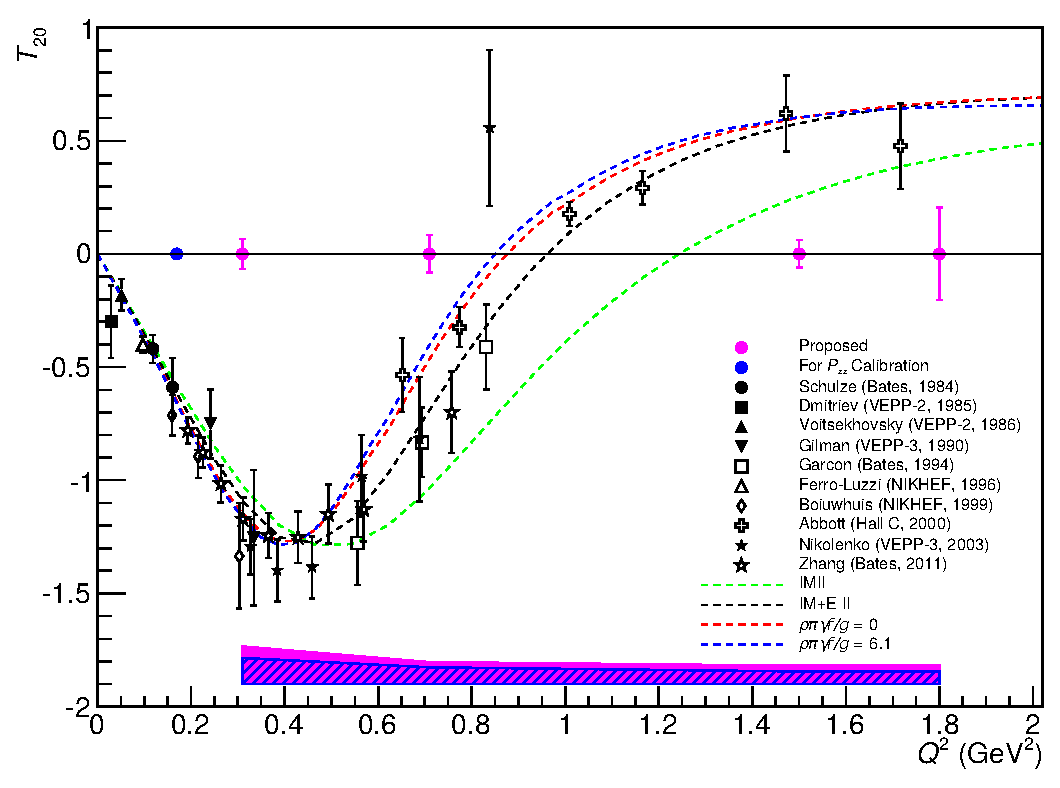
\includegraphics[width=\textwidth]{figs/plot_t20_fit.eps} 
\caption{\label{PROJ-T20}Projected uncertainties for the elastic tensor analyzing power $T_{20}$ with \productiondays days of beam time are shown alongside the world data~\cite{Holt:2012gg}. The point shown in blue, measured at $Q^2=0.2$~GeV$^2$ where $T_{20}$ is well known theoretically and experimentally, will be used as a calibration for $P_{zz}$, and can potentially be used to further reduce the leading systematic uncertainty as indicated by the blue-dashed band.
}
\end{center}
\end{figure}

\iffalse
\subsubsection{SHMS Angular Constraints}

It was recently pointed out that the SHMS is being built such that it would not be able to go to low angles without the magnets interfering with the beam dump~\cite{Moore:2014sxa}. In particular, angles below $\approx10^{\circ}$ would cause the beam to miss the dump. Although solutions have been proposed, including a passive system of adding extra iron to the magnet yokes and beam pipe to reduce field leakage, they have not yet been implemented. In the case that they are not installed by the time of running, we can utilize a slightly different set of kinematics that will cover most of the same $Q^2$ range as in Section~\ref{kinematics} but at lower beam energies and larger angles. Although less ideal, the physics motivation is still valid at the reduced kinematics and the rates still make for a compelling measurement, as shown in Table~\ref{RATES1-const} and Figs.~\ref{kincov-const}-\ref{PROJ-const}.

\begin{table}
\begin{center}
\begin{tabular}{cc|c|c|c|c|c|c}
 & & $E_0$ & $Q^2$    	& $E'$  &    $\theta_{e'}$  &  Rates   & PAC Time   \\
%& (GeV) & (GeV$^2$)  & (GeV)  &     (deg.)   &   (kHz)  & (hours) \\
& & (GeV) & (GeV$^2$)  & (GeV)  &     ($^{\circ}$)   &   (kHz)  & (Days) \\
%\multicolumn{2}{|c|}{$\times 10^{-2}$}
\hline\hline
% Spec  Set   E_0       Q^2      E'        Th         Rate      Time
SHMS & (S1') & 6.6	&  1.5	&  6.07	&    11.1  	&    0.13	&   25 \\
HMS  & (H1') & 6.6	&  1.8	&  5.96	&    12.3	&    0.09	&   25 \\  
%SHMS & (S2) & 4.4	&  0.6	&  4.20	&    10.1 	&    2.07	&   8 \\
SHMS & (S2') & 4.4	&  0.7	&  4.15	&    11.3 	&    0.90	&   8 \\
HMS  & (H2') & 4.4	&  0.8	&  4.11	&    12.2	&    0.80	&   8 \\
SHMS & (S3') & 2.2	&  0.2	&  2.15	&    10.9 	&    10.5	&   1 \\
HMS  & (H3') & 2.2	&  0.3	&  2.11	&    14.9	&    3.23	&   1 \\  
\hline\hline
\end{tabular}
\caption{\label{RATES1-const}Central kinematics if the SHMS is constrained to $>10^{\circ}$. The lowest settings (S3 and H3) are unchanged from Fig.~\ref{RATES1}.}
\end{center}
\end{table}

%


\begin{figure}
\begin{center}
%\includegraphics[width=\textwidth]{figs/Pzz_30_all_q2_w.eps}
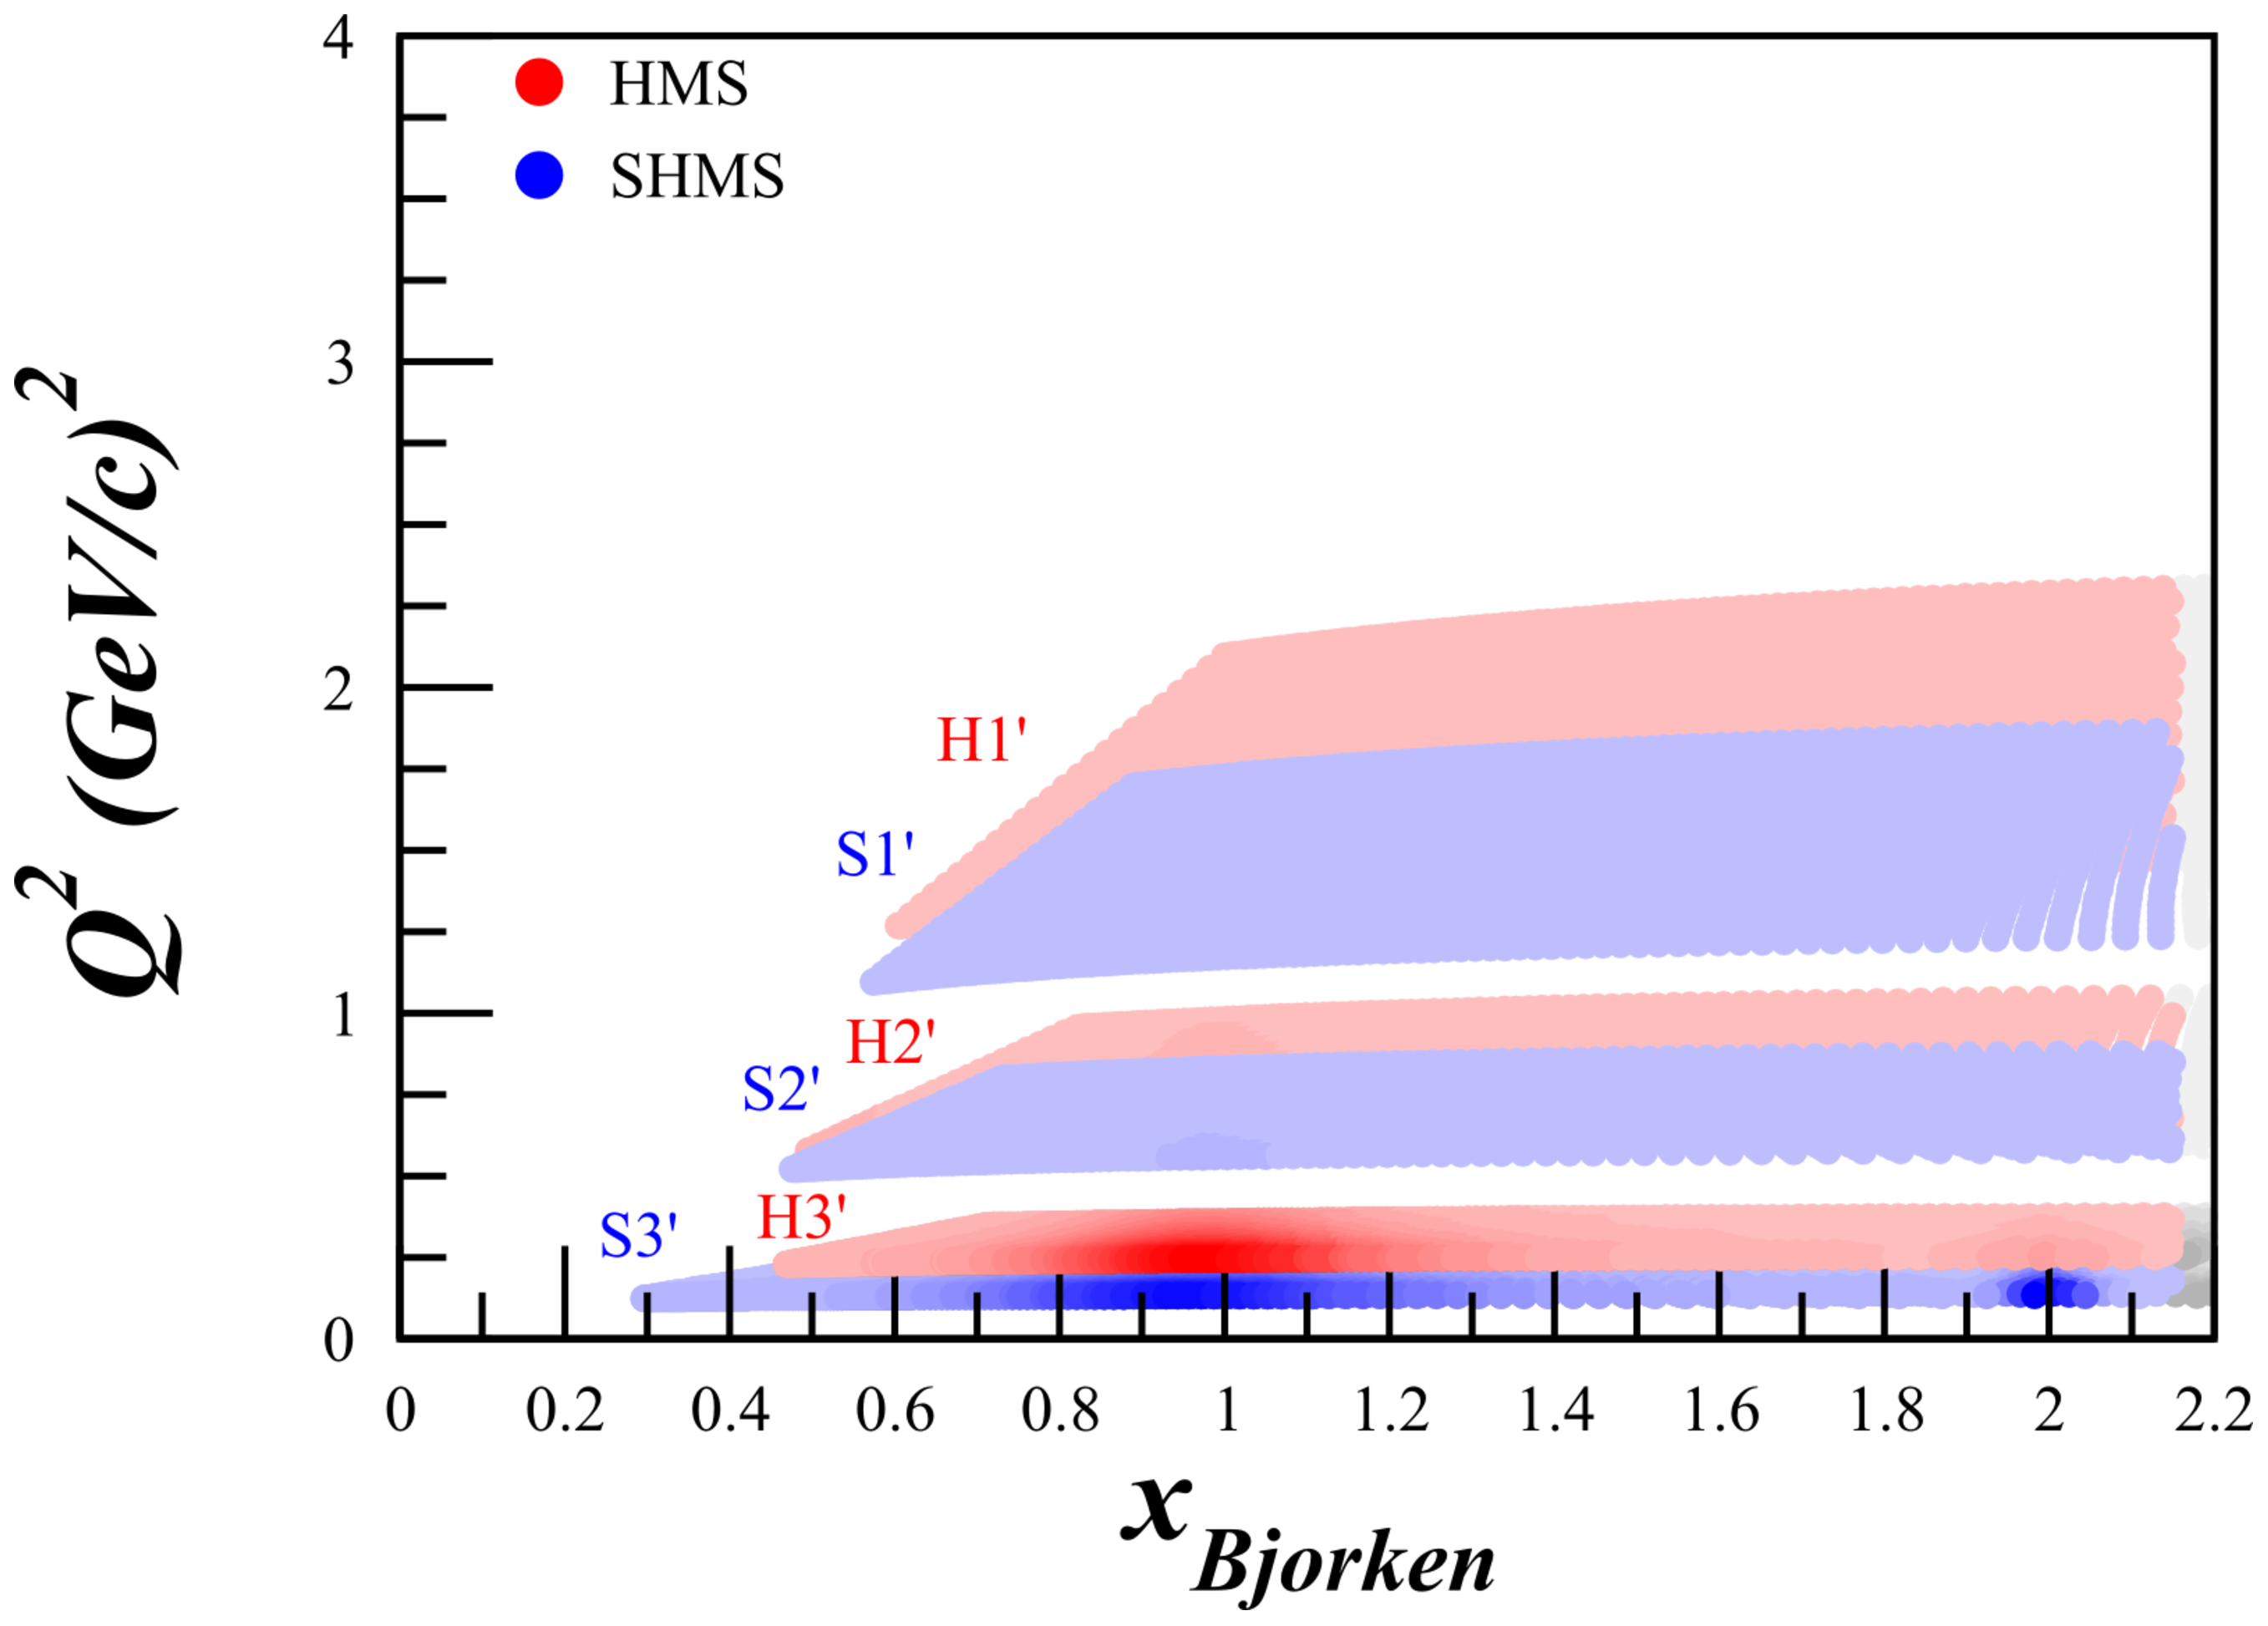
\includegraphics[width=0.49\textwidth]{figs/q2_shms_const.eps}

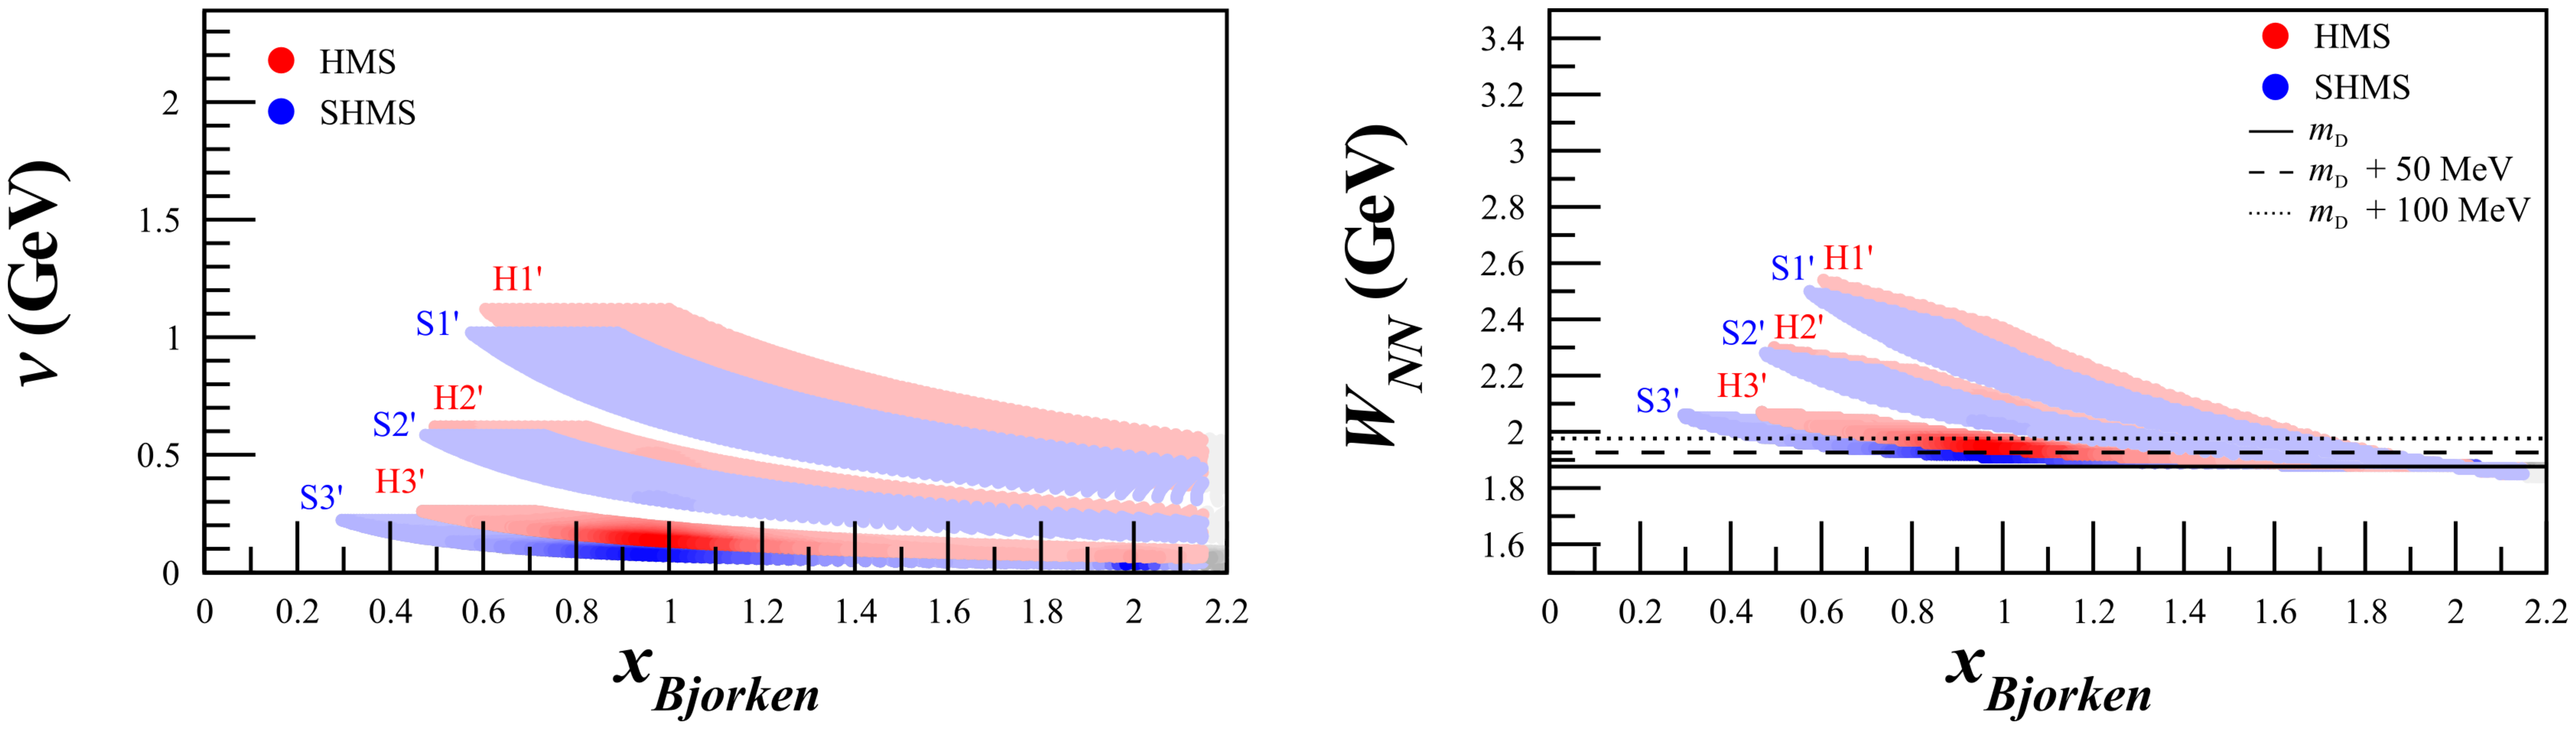
\includegraphics[width=\textwidth]{figs/nu_wnn_shms_const.eps}
%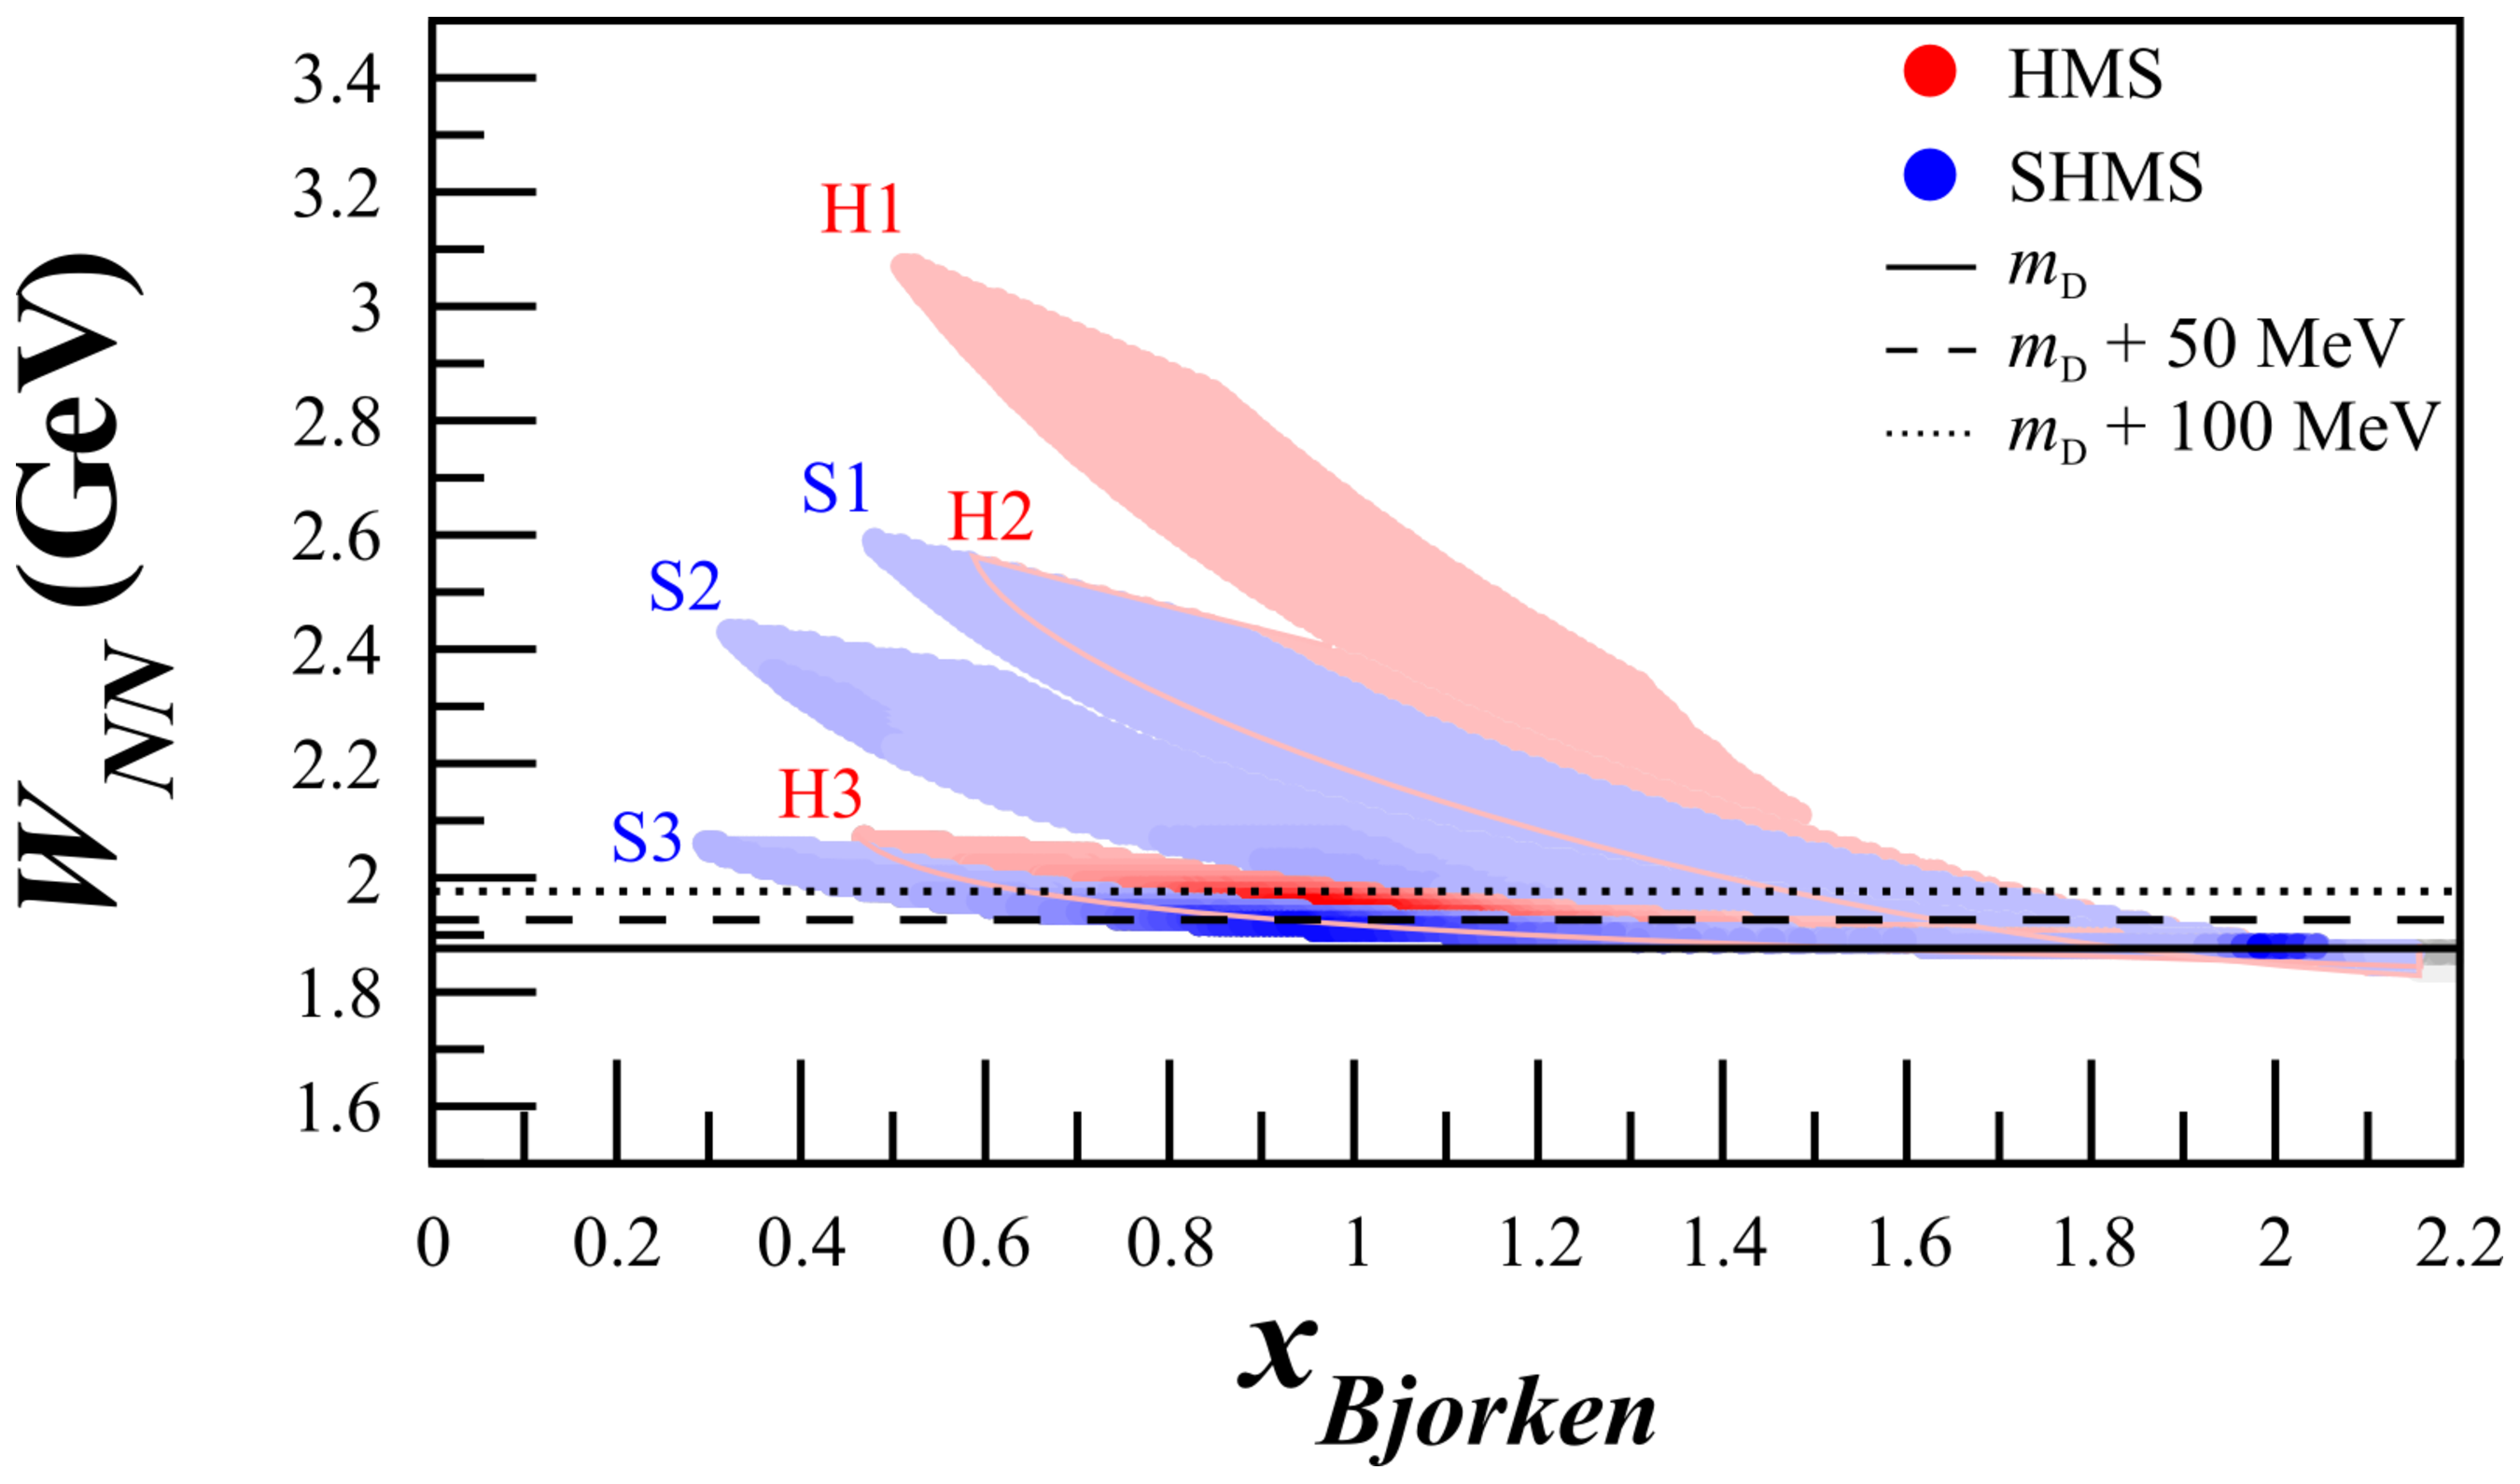
\includegraphics[width=0.49\textwidth]{figs/Pzz_30_all_wnn.eps} %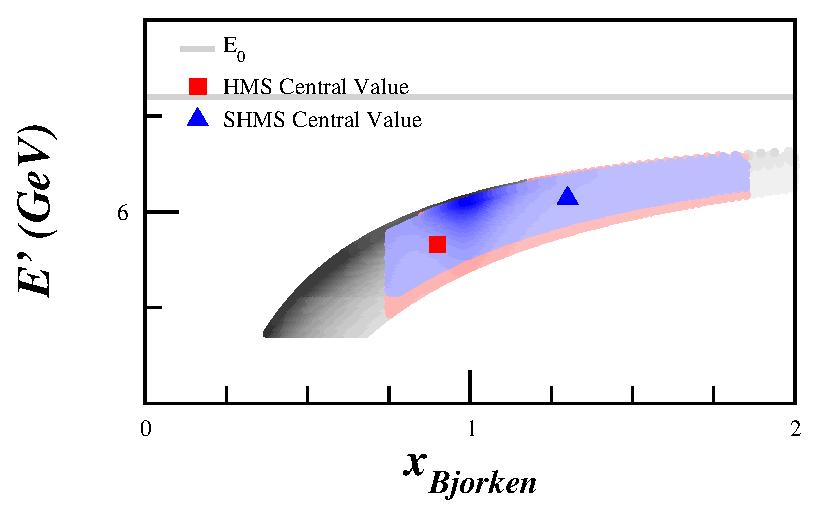
\includegraphics[width=0.49\textwidth]{figs/kine/Pzz_30_eprime.eps}
%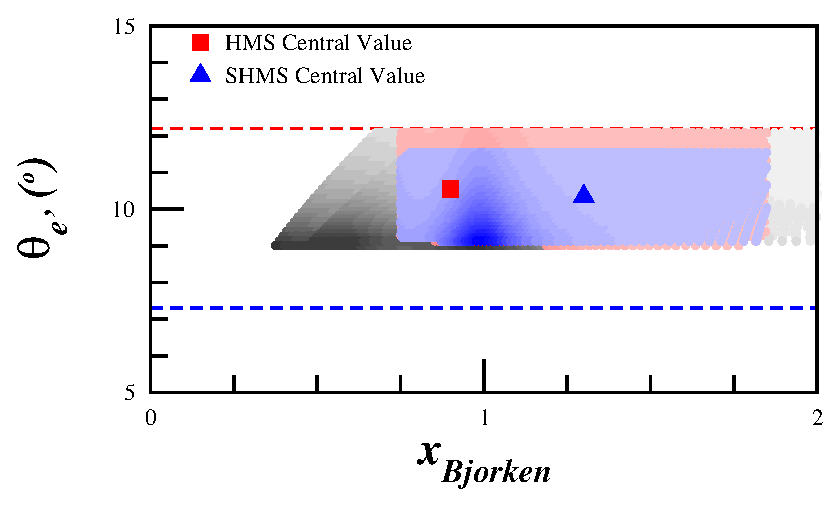
\includegraphics[width=0.49\textwidth]{figs/kine/Pzz_30_theta_eprime.eps}~~ 

\caption{\label{kincov-const} Kinematic coverage for the kinematics listed in Table~\ref{RATES1-const}, which can be achieved in the case that the SHMS is constrained to angles $>10^{\circ}$.}
\end{center}
\end{figure}



\begin{figure}
\begin{center}
\includegraphics[width=0.49\textwidth]{figs/Azz_shms_const.eps} \includegraphics[width=0.49\textwidth]{figs/t20_shms_const.eps} 
\caption{\label{PROJ-const}Projected uncertainties for the tensor asymmetry $A_{zz}$ and elastic analyzing power $T_{20}$ with \productiondays days of beam time using the constrained kinematics in Table~\ref{RATES1-const}.
}
\end{center}
\end{figure}
\fi